\newif\ifshowsolutions
\showsolutionstrue
\documentclass{article}
\usepackage{listings}
\usepackage{amsmath}
\usepackage{subfig}
\usepackage{amsthm}
\usepackage{amsmath}
\usepackage{amssymb}
\usepackage{graphicx}
\usepackage{mdwlist}
\usepackage{geometry}
\usepackage{titlesec}
\usepackage{palatino}
\usepackage{mathrsfs}
\usepackage{fancyhdr}
\usepackage{paralist}
\usepackage{todonotes}
\usepackage{tikz}
\usepackage{float} % Place figures where you ACTUALLY want it
\usepackage{comment} % A hack to toggle sections
\usepackage{ifthen}
\usepackage{mdframed}
\usepackage{verbatim}
\usepackage{listings}
\usepackage{bbm}
\usepackage{upquote} % Prevents backticks replacing single-quotes in verbatim
\usepackage[strings]{underscore}
\usepackage[colorlinks=true]{hyperref}
\usetikzlibrary{positioning,shapes,backgrounds}

\geometry{margin=1in}
\geometry{headheight=2in}
\geometry{top=2in}

\setlength{\marginparwidth}{2.15cm}
\setlength{\parindent}{0em}
\setlength{\parskip}{0.6\baselineskip}

\rhead{}
\lhead{}

% Spacing settings.
\titlespacing\section{0pt}{12pt plus 2pt minus 2pt}{0pt plus 2pt minus 2pt}
\titlespacing\subsection{0pt}{12pt plus 4pt minus 2pt}{0pt plus 2pt minus 2pt}
\titlespacing\subsubsection{0pt}{12pt plus 4pt minus 2pt}{0pt plus 2pt minus 2pt}
\renewcommand{\baselinestretch}{1.15}

% Shortcuts for commonly used operators.
\newcommand{\E}{\mathbb{E}}
\newcommand{\Var}{\operatorname{Var}}
\newcommand{\Cov}{\operatorname{Cov}}
\newcommand{\Bias}{\operatorname{Bias}}
\DeclareMathOperator{\argmin}{arg\,min}
\DeclareMathOperator{\argmax}{arg\,max}

% Do not number subsections and below.
\setcounter{secnumdepth}{1}

% Custom format subsection.
\titleformat*{\subsection}{\large\bfseries}

% Set up the problem environment.
\newcounter{problem}[section]
\newenvironment{problem}[1][]
  {\begingroup
    \setlength{\parskip}{0em}
    \refstepcounter{problem}\par\addvspace{1em}\textbf{Problem~\Alph{problem}\!
    \ifthenelse{\equal{#1}{}}{}{ [#1 points]}:}
  \endgroup}

% Set up the subproblem environment.
\newcounter{subproblem}[problem]
\newenvironment{subproblem}[1][]
  {\begingroup
    \setlength{\parskip}{0em}
    \refstepcounter{subproblem}\par\medskip\textbf{\roman{subproblem}.\!
    \ifthenelse{\equal{#1}{}}{}{ [#1 points]:}}
  \endgroup}

% Set up the teachers and materials commands.
\newcommand\teachers[1]
  {\begingroup
    \setlength{\parskip}{0em}
    \vspace{0.3em} \textit{\hspace*{2em} TAs responsible: #1} \par
  \endgroup}
\newcommand\materials[1]
  {\begingroup
    \setlength{\parskip}{0em}
    \textit{\hspace*{2em} Relevant materials: #1} \par \vspace{1em}
  \endgroup}

% Set up the hint environment.
\newenvironment{hint}[1][]
  {\begin{em}\textbf{Hint: }}
  {\end{em}}


% Set up the solution environment.
\ifshowsolutions
  \newenvironment{solution}[1][]
    {\par\medskip \begin{mdframed}\textbf{Solution~\Alph{problem}#1:} \begin{em}}
    {\end{em}\medskip\end{mdframed}\medskip}
  \newenvironment{subsolution}[1][]
    {\par\medskip \begin{mdframed}\textbf{Solution~\Alph{problem}#1.\roman{subproblem}:} \begin{em}}
    {\end{em}\medskip\end{mdframed}\medskip}
\else
  \excludecomment{solution}
  \excludecomment{subsolution}
\fi



%%%%%%%%%%%%%%%%%%%%%%%%%%%%%%
% HEADER
%%%%%%%%%%%%%%%%%%%%%%%%%%%%%%

\chead{%
  {\vbox{%
      \vspace{2mm}
      \large
      Machine Learning \& Data Mining \hfill
      Caltech CS/CNS/EE 155 \hfill \\[1pt]
      Homework 6\hfill
      March $1^\text{st}$ 2023 \\
    }
  }
}

\begin{document}
\pagestyle{fancy}

%%%%%%%%%%%%%%%%%%%%%%%%%%%%%%
% POLICIES
%%%%%%%%%%%%%%%%%%%%%%%%%%%%%%

\section*{Policies}
\begin{itemize}
  \item Due 9 PM, March $8^\text{th}$, via Gradescope.
  \item You are free to collaborate on all of the problems, subject to the collaboration policy stated in the syllabus. 
  \item You should submit all code used in the homework. We ask that you use Python 3.6+ for your code, and that you comment your code such that the TAs can follow along and run it without any issues.
\end{itemize}

\section*{Submission Instructions}
\begin{itemize}
   \item \textbf{In the report, include any images generated by your code along with your answers to the questions.} For instructions specifically pertaining to the Gradescope submission process, see \url{https://www.gradescope.com/get_started#student-submission}.
   
   \item Since we are only using Gradescope this year, we ask that you upload both your code and solution pdf together as a single pdf and mark each page with the problem number. There are various free online tools to combine pdfs. To download your code as a pdf from Jupyter notebook, you can navigate to File -$>$ Download as -$>$ "PDF via Latex" or alternatively download the Latex file and compile it yourself.
\end{itemize}

\newpage

\section{Probability Refresher [0 points]}

 \emph{This problem is a probability refresher and is worth $0$ points. It should take you no more than 2-4 minutes to solve for each part. If you find that you are taking more time, you should probably watch the Probability recitation.}\\

\problem[0] If $X, Y \sim \mathcal{N}(0, 1)$, compute $\Pr[X < \frac{Y}{\sqrt{2}}]$.\\


\begin{solution}
\end{solution}

\vspace{0.5cm}

\problem[0] If $X, Y \sim \mathcal{N}(0, 1)$, compute $\Pr[X+Y>0 | X>0]$. \\

\begin{solution}
\end{solution}

\vspace{0.5cm}

\problem[0] Prove that $\sigma$-algebras are closed under finitely many intersections. Hint: Recall that they are closed under finitely many unions and complements.\\

\begin{solution}
\qedhere
\end{solution}

\vspace{0.5cm}

\problem[0] If $X$ is a continuous random variable that takes on values in the range $(0,\infty)$, and $Y$ is another random variable such that the marginal density of $X$ and $Y$ is given by
\[f_{X,Y}(x,y) = \frac{1}{y} e^{-x/y}e^{-y}\]
What is the probability distribution function of $Y$? \\

\begin{solution}
\end{solution}

\newpage

%%%%%%%%%%%%%%%%%%%%%%%%%%%%%%
% PROBLEM 1
%%%%%%%%%%%%%%%%%%%%%%%%%%%%%%

\section{Class-Conditional Densities for Binary Data [25 Points]}
This problem will test your understanding of probabilistic models, especially Naive Bayes.
Consider a generative classifier for $C$ classes, with class conditional density $p(x | y)$ and a uniform class prior $p(y)$. Suppose all the $D$ features are binary, $x_j \in \{0, 1 \}$. If we assume all of the features are conditionally independent, as in Naive Bayes, we can write:
$$p(x \mid y = c) = \prod_{j=1}^D P(x_j \mid y = c) $$
This requires storing $DC$ parameters. 

Now consider a different model, which we will call the `full' model, in which all the features are fully \textit{dependent}.

\problem[5]Use the chain rule of probability to factorize $p(x \mid y)$, and let $\theta_{xjc} = P(x_j | x_{1, \ldots, j - 1}, y = c)$. Assuming we store each $\theta_{xjc}$, how many parameters are needed to represent this factorization? Use big-O notation.

\begin{solution} % Thanks to Michael for pointing this out
  \begin{align*}
    p(x \mid y = c) &= P(x_1, \dots, x_D \mid y = c) \\
      &= \theta_{xDc} P(x_1, \dots, x_{D-1} \mid y = c) \\
      &= \prod_{j=1}^D \theta{xjc}
  \end{align*}

  There are $DC$ terms in the product, but $\theta_{xjc}$ depends on $j - 1$ other $x$ values, so it uses $2^{j-1}$ parameters.
  So the number of parameters is $C \sum_{j=1}^D 2^{j-1} = C (2^D - 1)$, which is $O(C \cdot 2^D)$.
\end{solution}

\problem[5] Assume we did no such factorization, and just used the conditional probability $p(x \mid y = c)$. How many parameters would we need to estimate in order be able to compute $p(x | y = c)$ for arbitrary $x$ and $c$? How does this compare to your answer from the previous part? Again, use big-O notation.

\begin{solution}
  Given $2^D$ possible values for $x$ and $C$ values for $c$, we have $O(C \cdot 2^D)$ again.
\end{solution}

\problem[2] Assume the number of features $D$ is fixed. Let there be $N$ training cases. If the sample size $N$ is very small, which model (Naive Bayes or full) is likely to give lower test set error, and why?

\begin{solution}
  Naive Bayes is likely to give the lower test error, because as long as $N < 2^D$ the full model can just memorize the entire training set, so it will overfit.
\end{solution}

\problem[2] If the sample size $N$ is very large, which model (Naive Bayes or full) is likely to give lower test set error, and why?
\begin{solution}
  With very large $N$ the full model is likely to give lower test error, because it has higher capacity and can thus learn more from the training set.
\end{solution}

\problem[11] Assume all the parameter estimates have been computed. What is the computational complexity of making a prediction, i.e. computing $p(y \mid x)$, using Naive Bayes for a single test case? What is the computation complexity of making a prediction with the full model? For the full-model case, assume that converting a $D$-bit vector to an array index is an $O(D)$ operation.  Also, recall that we have assumed a uniform class prior. 

\begin{solution}
  Assuming a uniform class prior,
  $$ p(y \mid x) = \frac{p(y, x)}{p(x)} = \frac{p(x \mid y) p(y)}{p(x)} \propto p(x \mid y) $$

  For Naive Bayes, we have to look up and multiply $D$ parameters for each of the $C$ classes, so the complexity is $O(DC)$.

  For the full model, we have to convert $x$ into an array index (which is $O(D)$) for each of the $C$ classes, so the complexity is $O(DC)$ again.
\end{solution}


\newpage
\section{Sequence Prediction [75 Points]}

In this problem, we will explore some of the various algorithms associated with Hidden Markov Models (HMMs), as discussed in lecture.  For these problems, make sure you are \textbf{using Python 3} to implement the algorithms. Please see the HMM notes posted on the course website---they will be helpful for this problem!

\subsection{Sequence Prediction}

These next few problems will require extensive coding, so be sure to start early! We provide you with eight different files:
\begin{itemize}
  \item You will write all your code in \texttt{HMM.ipynb}, within the appropriate functions where indicated by "TODO" in the comments. There is no need to modify anything else aside from what is indicated. There should be no need to write additional functions or use NumPy in your implementation, but feel free to do so if you would like. 
\end{itemize}

The supplementary data folder contains 6 files titled \texttt{sequence_data0.txt}, \texttt{sequence_data1.txt}, ... , \texttt{sequence_data5.txt}. Each file specifies a \textbf{trained} HMM. The first row contains two tab-delimited numbers: the number of states $Y$ and the number of types of observations $X$ (i.e. the observations are $0, 1, . . . , X - 1$). The next $Y$ rows of $Y$ tab-delimited floating-point numbers describe the state transition matrix. Each row represents the current state, each column represents a state to transition to, and each entry represents the probability of that transition occurring. The next $Y$ rows of $X$ tab-delimited floating-point numbers describe the output emission matrix, encoded analogously to the state transition matrix. The file ends with 5 possible emissions from that HMM. \\

The supplementary data folder also contains one additional file titled \texttt{ron.txt}. This is used in problems 2C and 2D and is explained in greater detail there. 
\indent\problem[10] % indent for consistency
For each of the six trained HMMs, find the max-probability state sequence for each of the five input sequences at the end of the corresponding file. To complete this problem, you will have to implement the Viterbi algorithm. Write your implementation well, as we will be reusing it in a later problem. See the end of problem 2B for a big hint!

Show your results on the 6 files. (Copy-pasting the results of under the "Part A" heading of \texttt{HMM.ipynb} suffices.)
\begin{solution}
  \href{https://drive.google.com/file/d/1CgGDvZ95ua7JDxOb4WkoU3T8oF0RCYgW/view?usp=sharing}{Colab notebook}

  \begin{verbatim}
File #0:
Emission Sequence             Max Probability State Sequence
######################################################################
25421                         31033                         
01232367534                   22222100310                   
5452674261527433              1031003103222222              
7226213164512267255           1310331000033100310           
0247120602352051010255241     2222222222222222222222103     

File #1:
Emission Sequence             Max Probability State Sequence
######################################################################
77550                         22222                         
7224523677                    2222221000                    
505767442426747               222100003310031               
72134131645536112267          10310310000310333100          
4733667771450051060253041     2221000003222223103222223     

File #2:
Emission Sequence             Max Probability State Sequence
######################################################################
60622                         11111                         
4687981156                    2100202111                    
815833657775062               021011111111111               
21310222515963505015          02020111111111111021          
6503199452571274006320025     1110202111111102021110211     

File #3:
Emission Sequence             Max Probability State Sequence
######################################################################
13661                         00021                         
2102213421                    3131310213                    
166066262165133               133333133133100               
53164662112162634156          20000021313131002133          
1523541005123230226306256     1310021333133133313133133     

File #4:
Emission Sequence             Max Probability State Sequence
######################################################################
23664                         01124                         
3630535602                    0111201112                    
350201162150142               011244012441112               
00214005402015146362          11201112412444011112          
2111266524665143562534450     2012012424124011112411124     

File #5:
Emission Sequence             Max Probability State Sequence
######################################################################
68535                         10111                         
4546566636                    1111111111                    
638436858181213               110111010000011               
13240338308444514688          00010000000111111100          
0111664434441382533632626     2111111111111100111110101
  \end{verbatim}
\end{solution}
\indent\problem[17] % indent for consistency
For each of the six trained HMMs, find the probabilities of emitting the five input sequences at the end of the corresponding file. To complete this problem, you will have to implement the Forward algorithm and the Backward algorithm. You may assume that the initial state is randomly selected along a uniform distribution. Again, write your implementation well, as we will be reusing it in a later problem. \\

Note that the probability of emitting an input sequence can be found by using either the $\alpha$ vectors from the Forward algorithm or the $\beta$ vectors from the Backward algorithm. You don't need to worry about this, as it is done for you in \texttt{probability\_alphas()} and \texttt{probability\_betas()}.

Implement the Forward algorithm. Show your results on the 6 files. \\
Implement the Backward algorithm. Show your results on the 6 files. \\

After you complete problems 2A and 2B, you can compare your results for the file titled \texttt{sequence_data0.txt} with the values given in the table below:
\begin{center}
  \begin{tabular}{ l | l |l | l }
Dataset & Emission Sequence & Max-probability State Sequence & Probability of Sequence  \\ \hline
0 & 25421                      &  31033           & 4.537e-05\\
0 & 01232367534                &  22222100310       & 1.620e-11\\
0 & 5452674261527433           &  1031003103222222      & 4.348e-15\\
0 & 7226213164512267255        &  1310331000033100310   & 4.739e-18\\
0 & 0247120602352051010255241  &  2222222222222222222222103 & 9.365e-24
 \\ \hline
 \end{tabular}
\end{center}

\begin{solution}
  Forward algorithm:
  \begin{verbatim}
File #0:
Emission Sequence             Probability of Emitting Sequence
######################################################################
25421                         4.537e-05 
01232367534                   1.620e-11 
5452674261527433              4.348e-15 
7226213164512267255           4.739e-18 
0247120602352051010255241     9.365e-24 

File #1:
Emission Sequence             Probability of Emitting Sequence
######################################################################
77550                         1.181e-04 
7224523677                    2.033e-09 
505767442426747               2.477e-13 
72134131645536112267          8.871e-20 
4733667771450051060253041     3.740e-24 

File #2:
Emission Sequence             Probability of Emitting Sequence
######################################################################
60622                         2.088e-05 
4687981156                    5.181e-11 
815833657775062               3.315e-15 
21310222515963505015          5.126e-20 
6503199452571274006320025     1.297e-25 

File #3:
Emission Sequence             Probability of Emitting Sequence
######################################################################
13661                         1.732e-04 
2102213421                    8.285e-09 
166066262165133               1.642e-12 
53164662112162634156          1.063e-16 
1523541005123230226306256     4.535e-22 

File #4:
Emission Sequence             Probability of Emitting Sequence
######################################################################
23664                         1.141e-04 
3630535602                    4.326e-09 
350201162150142               9.793e-14 
00214005402015146362          4.740e-18 
2111266524665143562534450     5.618e-22 

File #5:
Emission Sequence             Probability of Emitting Sequence
######################################################################
68535                         1.322e-05 
4546566636                    2.867e-09 
638436858181213               4.323e-14 
13240338308444514688          4.629e-18 
0111664434441382533632626     1.440e-22 
  \end{verbatim}

  Backward algorithm:
  \begin{verbatim}
File #0:
Emission Sequence             Probability of Emitting Sequence
######################################################################
25421                         4.537e-05 
01232367534                   1.620e-11 
5452674261527433              4.348e-15 
7226213164512267255           4.739e-18 
0247120602352051010255241     9.365e-24 

File #1:
Emission Sequence             Probability of Emitting Sequence
######################################################################
77550                         1.181e-04 
7224523677                    2.033e-09 
505767442426747               2.477e-13 
72134131645536112267          8.871e-20 
4733667771450051060253041     3.740e-24 

File #2:
Emission Sequence             Probability of Emitting Sequence
######################################################################
60622                         2.088e-05 
4687981156                    5.181e-11 
815833657775062               3.315e-15 
21310222515963505015          5.126e-20 
6503199452571274006320025     1.297e-25 

File #3:
Emission Sequence             Probability of Emitting Sequence
######################################################################
13661                         1.732e-04 
2102213421                    8.285e-09 
166066262165133               1.642e-12 
53164662112162634156          1.063e-16 
1523541005123230226306256     4.535e-22 

File #4:
Emission Sequence             Probability of Emitting Sequence
######################################################################
23664                         1.141e-04 
3630535602                    4.326e-09 
350201162150142               9.793e-14 
00214005402015146362          4.740e-18 
2111266524665143562534450     5.618e-22 

File #5:
Emission Sequence             Probability of Emitting Sequence
######################################################################
68535                         1.322e-05 
4546566636                    2.867e-09 
638436858181213               4.323e-14 
13240338308444514688          4.629e-18 
0111664434441382533632626     1.440e-22 
  \end{verbatim}
\end{solution}

\subsection{HMM Training}
Ron is an avid music listener, and his genre preferences at any given time depend on his mood. Ron's possible moods are happy, mellow, sad, and angry. Ron experiences one mood per day (as humans are known to do) and chooses one of ten genres of music to listen to that day depending on his mood. \\

Ron's roommate, who is known to take to odd hobbies, is interested in how Ron's mood affects his music selection, and thus collects data on Ron's mood and music selection for six years (2190 data points). This data is contained in the supplementary file \texttt{ron.txt}. Each row contains two tab-delimited strings: Ron's mood and Ron's genre preference that day. The data is split into 12 sequences, each corresponding to half a year's worth of observations. The sequences are separated by a row containing only the character \texttt{-}.
\noindent\problem[10] % indent for consistency
Use a single M-step to train a supervised Hidden Markov Model on the data in \texttt{ron.txt}.

After you implement 2C, please compare your output transition and observation matrices with the state transition and output emission matrices below. You should make sure your outputs match before continuing.

Transition matrix = \small $\begin{pmatrix}
    2.833\text{e-}01 & 4.714\text{e-}01 & 1.310\text{e-}01 & 1.143\text{e-}01 \\
    2.321\text{e-}01 & 3.810\text{e-}01 & 2.940\text{e-}01 & 9.284\text{e-}02 \\
    1.040\text{e-}01 & 9.760\text{e-}02 & 3.696\text{e-}01 & 4.288\text{e-}01 \\
    1.883\text{e-}01 & 9.903\text{e-}02 & 3.052\text{e-}01 & 4.075\text{e-}01 
\end{pmatrix}$
\normalsize

Observation Matrix =

\small
$\begin{pmatrix}
1.486\text{e-}01 & 2.288\text{e-}01 & 1.533\text{e-}01 & 1.179\text{e-}01 & 4.717\text{e-}02 & 5.189\text{e-}02 & 2.830\text{e-}02 & 1.297\text{e-}01 & 9.198\text{e-}02 & 2.358\text{e-}03 \\
1.062\text{e-}01 & 9.653\text{e-}03 & 1.931\text{e-}02 & 3.089\text{e-}02 & 1.699\text{e-}01 & 4.633\text{e-}02 & 1.409\text{e-}01 & 2.394\text{e-}01 & 1.371\text{e-}01 & 1.004\text{e-}01 \\
1.194\text{e-}01 & 4.299\text{e-}02 & 6.529\text{e-}02 & 9.076\text{e-}02 & 1.768\text{e-}01 & 2.022\text{e-}01 & 4.618\text{e-}02 & 5.096\text{e-}02 & 7.803\text{e-}02 & 1.274\text{e-}01 \\
1.694\text{e-}01 & 3.871\text{e-}02 & 1.468\text{e-}01 & 1.823\text{e-}01 & 4.839\text{e-}02 & 6.290\text{e-}02 & 9.032\text{e-}02 & 2.581\text{e-}02 & 2.161\text{e-}01 & 1.935\text{e-}02 
\end{pmatrix}$
\normalsize
\medskip

\begin{solution}
  Our outputs match the matrices given.

  \begin{verbatim}
Transition Matrix:
######################################################################
2.833e-01   4.714e-01   1.310e-01   1.143e-01   
2.321e-01   3.810e-01   2.940e-01   9.284e-02   
1.040e-01   9.760e-02   3.696e-01   4.288e-01   
1.883e-01   9.903e-02   3.052e-01   4.075e-01   


Observation Matrix:  
######################################################################
1.486e-01   2.288e-01   1.533e-01   1.179e-01   4.717e-02   5.189e-02   2.830e-02   1.297e-01   9.198e-02   2.358e-03   
1.062e-01   9.653e-03   1.931e-02   3.089e-02   1.699e-01   4.633e-02   1.409e-01   2.394e-01   1.371e-01   1.004e-01   
1.194e-01   4.299e-02   6.529e-02   9.076e-02   1.768e-01   2.022e-01   4.618e-02   5.096e-02   7.803e-02   1.274e-01   
1.694e-01   3.871e-02   1.468e-01   1.823e-01   4.839e-02   6.290e-02   9.032e-02   2.581e-02   2.161e-01   1.935e-02
  \end{verbatim}
\end{solution}
\indent\problem[15] % indent for consistency
Now suppose that Ron has a third roommate who is also interested in how Ron's mood affects his music selection. This roommate is lazier than the other one, so he simply steals the first roommate's data. Unfortunately, he only manages to grab half the data, namely, Ron's choice of music for each of the 2190 days.

In this problem, we will train an unsupervised Hidden Markov Model on this data. Recall that unsupervised HMM training is done using the Baum-Welch algorithm and will require repeated EM steps. For this problem, we will use 4 hidden states and run the algorithm for 1000 iterations. The transition and observation matrices are initialized for you in the helper functions \texttt{supervised\_learning()} and \texttt{unsupervised\_learning()} such that they are random and normalized.

What are the learned state transition and output emission matrices?

Below are the transition and observation matrices for the unsupervised Hidden Markov Model at the zero-th iteration.

Transition Matrix = \small $\begin{pmatrix}
2.003\text{e-}01 & 3.720\text{e-}01 & 5.642\text{e-}02 & 3.713\text{e-}01\\
1.581\text{e-}01 & 2.147\text{e-}01 & 4.197\text{e-}01 & 2.075\text{e-}01\\
2.941\text{e-}01 & 1.475\text{e-}02 & 4.032\text{e-}01 & 2.880\text{e-}01\\
1.759\text{e-}01 & 4.205\text{e-}01 & 1.617\text{e-}01 & 2.419\text{e-}01 
\end{pmatrix}$
\normalsize

Observation Matrix =

\small
$\begin{pmatrix}
2.585\text{e-}02 & 7.773\text{e-}02 & 3.923\text{e-}02 & 5.058\text{e-}02 & 1.447\text{e-}01 & 5.407\text{e-}02 & 9.356\text{e-}02 & 1.891\text{e-}01 & 1.854\text{e-}01 & 1.398\text{e-}01\\
9.821\text{e-}02 & 5.024\text{e-}02 & 2.915\text{e-}02 & 1.760\text{e-}01 & 9.364\text{e-}02 & 2.102\text{e-}02 & 1.131\text{e-}01 & 1.409\text{e-}01 & 1.112\text{e-}01 & 1.664\text{e-}01\\
8.272\text{e-}03 & 1.104\text{e-}01 & 9.597\text{e-}02 & 1.303\text{e-}02 & 1.340\text{e-}01 & 1.781\text{e-}01 & 1.239\text{e-}01 & 5.434\text{e-}02 & 1.755\text{e-}01 & 1.065\text{e-}01\\
1.028\text{e-}01 & 1.516\text{e-}01 & 2.977\text{e-}02 & 1.650\text{e-}01 & 1.375\text{e-}01 & 1.584\text{e-}01 & 3.856\text{e-}02 & 1.615\text{e-}01 & 3.851\text{e-}02 & 1.641\text{e-}02 
\end{pmatrix}$
\normalsize
\medskip

Below are the transition and observation matrices for the unsupervised Hidden Markov Model at the first iteration.

Transition Matrix = \small $\begin{pmatrix}
1.887\text{e-}01 & 3.750\text{e-}01 & 5.354\text{e-}02 & 3.828\text{e-}01\\
1.516\text{e-}01 & 2.204\text{e-}01 & 4.083\text{e-}01 & 2.196\text{e-}01\\
2.832\text{e-}01 & 1.556\text{e-}02 & 3.924\text{e-}01 & 3.089\text{e-}01\\
1.647\text{e-}01 & 4.254\text{e-}01 & 1.559\text{e-}01 & 2.540\text{e-}01   
\end{pmatrix}$
\normalsize

Observation Matrix =

\small
$\begin{pmatrix}
6.272\text{e-}02 & 5.705\text{e-}02 & 8.345\text{e-}02 & 5.738\text{e-}02 & 1.380\text{e-}01 & 5.191\text{e-}02 & 8.730\text{e-}02 & 1.572\text{e-}01 & 2.127\text{e-}01 & 9.231\text{e-}02\\
2.152\text{e-}01 & 3.537\text{e-}02 & 5.388\text{e-}02 & 1.786\text{e-}01 & 8.065\text{e-}02 & 1.888\text{e-}02 & 8.992\text{e-}02 & 1.053\text{e-}01 & 1.168\text{e-}01 & 1.054\text{e-}01\\
1.988\text{e-}02 & 8.040\text{e-}02 & 1.846\text{e-}01 & 1.378\text{e-}02 & 1.243\text{e-}01 & 1.626\text{e-}01 & 1.081\text{e-}01 & 4.324\text{e-}02 & 1.937\text{e-}01 & 6.944\text{e-}02\\
2.222\text{e-}01 & 1.001\text{e-}01 & 5.614\text{e-}02 & 1.652\text{e-}01 & 1.169\text{e-}01 & 1.376\text{e-}01 & 3.193\text{e-}02 & 1.205\text{e-}01 & 3.943\text{e-}02 & 9.930\text{e-}03 
\end{pmatrix}$
\normalsize
\medskip

Below are the transition and observation matrices for the unsupervised Hidden Markov Model at the final iteration (iteration 1000).

Transition Matrix = \small $\begin{pmatrix}
    4.345\text{e-}01 & 1.559\text{e-}01 & 9.612\text{e-}02 & 3.134\text{e-}01\\
    5.904\text{e-}15 & 2.996\text{e-}01 & 7.004\text{e-}01 & 1.328\text{e-}11\\
    5.219\text{e-}01 & 3.828\text{e-}18 & 2.259\text{e-}01 & 2.522\text{e-}01\\
    5.016\text{e-}03 & 3.679\text{e-}01 & 7.971\text{e-}03 & 6.191\text{e-}01 
\end{pmatrix}$ 
\normalsize

Observation Matrix =

\small
$\begin{pmatrix}
    2.235\text{e-}01 & 8.353\text{e-}09 & 7.603\text{e-}02 & 9.263\text{e-}02 & 2.315\text{e-}02 & 1.023\text{e-}02 & 1.273\text{e-}01 & 3.294\text{e-}01 & 1.288\text{e-}10 & 1.177\text{e-}01\\ 
    2.260\text{e-}01 & 3.339\text{e-}05 & 7.427\text{e-}14 & 2.039\text{e-}01 & 3.226\text{e-}02 & 1.151\text{e-}01 & 1.575\text{e-}01 & 3.954\text{e-}30 & 8.256\text{e-}02 & 1.828\text{e-}01\\  
    3.403\text{e-}02 & 1.351\text{e-}01 & 1.900\text{e-}01 & 5.006\text{e-}02 & 2.247\text{e-}01 & 2.150\text{e-}05 & 6.462\text{e-}02 & 2.926\text{e-}02 & 2.723\text{e-}01 & 3.988\text{e-}65\\   
    8.931\text{e-}02 & 1.173\text{e-}01 & 1.035\text{e-}01 & 9.344\text{e-}02 & 1.505\text{e-}01 & 2.098\text{e-}01 & 9.588\text{e-}07 & 7.679\text{e-}02 & 1.594\text{e-}01 & 1.312\text{e-}07   
\end{pmatrix}$
\normalsize
\medskip

Please use these outputs to check your code.

\begin{solution}
  Our outputs match the matrices given.
  \begin{verbatim}
Transition Matrix:
######################################################################
4.345e-01   1.559e-01   9.612e-02   3.134e-01   
5.904e-15   2.996e-01   7.004e-01   1.328e-11   
5.219e-01   3.828e-18   2.259e-01   2.522e-01   
5.016e-03   3.679e-01   7.971e-03   6.191e-01   


Observation Matrix:  
######################################################################
2.235e-01   8.353e-09   7.603e-02   9.263e-02   2.315e-02   1.023e-02   1.273e-01   3.294e-01   1.288e-10   1.177e-01   
2.260e-01   3.339e-05   7.427e-14   2.039e-01   3.226e-02   1.151e-01   1.575e-01   3.954e-30   8.256e-02   1.828e-01   
3.403e-02   1.351e-01   1.900e-01   5.006e-02   2.247e-01   2.150e-05   6.462e-02   2.926e-02   2.723e-01   3.988e-65   
8.931e-02   1.173e-01   1.035e-01   9.344e-02   1.505e-01   2.098e-01   9.588e-07   7.679e-02   1.594e-01   1.312e-07
  \end{verbatim}
\end{solution}

\problem[5] How do the transition and emission matrices from 2C and 2D compare? Which do you think provides a more accurate representation of Ron's moods and how they affect his music choices? Justify your answer. Suggest one way that we may be able to improve the method (supervised or unsupervised) that you believe produces the less accurate representation. 

\begin{solution}
  The unsupervised algorithm produced sparser matrices, where some of the entries are nearly 0 in both the transition and observation matrices.

  By looking at the observation matrices and the genre map, we saw that the supervised model produces a distribution over genres that makes intuitive sense to us (e.g. angry -> rap, metal, rock; happy -> pop, house, rock).
  The unsupervised model seemed to predict unrelated genres for a given state (for example rock, folk, and classical being the most likely from state 1).

  \begin{tabular}{c c}
    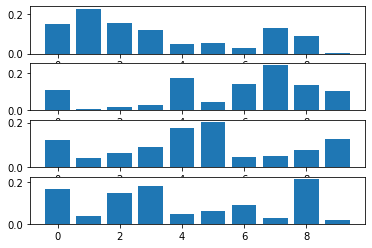
\includegraphics[width=0.45\textwidth]{images/2e_supervised.png} &
    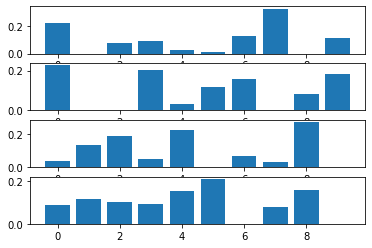
\includegraphics[width=0.45\textwidth]{images/2e_unsupervised.png} \\
    Supervised Model & Unsupervised Model
  \end{tabular}

  For improving the unsupervised model, we can gather more data, increase the number of epochs, or try more/fewer hidden states.
\end{solution}

\subsection{Sequence Generation}
Hidden Markov Models fall under the umbrella of generative models and therefore can be used to not only predict sequential data, but also to generate it. 
\problem[5] Load the trained HMMs from the files titled \texttt{sequence_data0.txt}, $\ldots$ , \texttt{sequence_data5.txt}. Use the six models to probabilistically generate five sequences of emissions from each model, each of length 20. Show your results. 

\begin{solution}
  \begin{verbatim}
File #0:
Generated Emission            
######################################################################
77420454341752715750          
72457572640525742077          
77646442257647445465          
65244754502514721023          
62772345127414575542          

File #1:
Generated Emission            
######################################################################
77420454341752715750          
72457572640525742077          
77646442257647445465          
65244754502514721023          
62772345127414575542          

File #2:
Generated Emission            
######################################################################
99540565323972926751          
72568781750637954077          
87836321467659227365          
75123966712525932224          
73993455259226683524          

File #3:
Generated Emission            
######################################################################
66330354312651605630          
61256660620512622066          
36624310326546115244          
53012653511322620012          
41663243236113433312          

File #4:
Generated Emission            
######################################################################
66320463212652606630          
62465660630514622066          
66535310256636115344          
53012654502324621122          
32662232136214462312          

File #5:
Generated Emission            
######################################################################
88341483323863806630          
63468680640635834166          
88836320456648115354          
63022865512334821234          
62883443238214483314          
  \end{verbatim}
\end{solution}

\subsection{Visualization \& Analysis}

Once you have implemented the above, load and run \texttt{2_notebook.ipynb}. In this notebook, you will apply the HMM you have implemented to the Constitution. There is no coding required for this part, only analysis. To run the notebook, however, you will likely need to install the \texttt{wordcloud} package. Please refer to the provided installation instructions if you get an error when running \texttt{pip install wordcloud}.

Answer the following problems in the context of the visualizations in the notebook.

\indent\problem[3] % indent for consistency
What can you say about the sparsity of the trained $A$ and $O$ matrices? How does this sparsity affect the transition and observation behaviour at each state?
\begin{solution}
  
  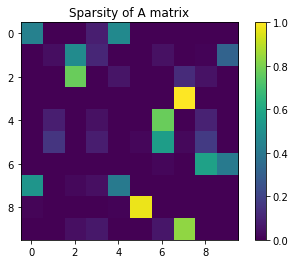
\includegraphics[width=0.45\textwidth]{images/sparsity_a.png}
  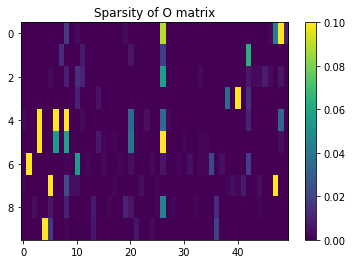
\includegraphics[width=0.45\textwidth]{images/sparsity_o.png}

  They're very sparse.
  This means that a given state is fairly certain for what observation it will produce and what state it will transition to.
\end{solution}

\indent\problem[5] % indent for consistency
How do the sample emission sentences from the HMM change as the number of hidden states is increased? What happens in the special case where there is only one hidden state? In general, when the number of hidden states is unknown while training an HMM for a fixed observation set, can we increase the training data likelihood by allowing more hidden states?

\begin{solution}
  None of the sentences make any sense, but the ones with more hidden states are able to make 2-3 word phrases that sound plausible.

  The 1 state model just randomly selects words according to their frequency in the text.

  In general, adding more hidden states will increase the training data likelihood because adding states can capture more complex patterns in the training data.
\end{solution}


\indent\problem[5] % indent for consistency
Pick a state that you find semantically meaningful, and analyze this state and its wordcloud. What does this state represent? How does this state differ from the other states? Back up your claim with a few key words from the wordcloud.
\begin{solution}
  
  
\includegraphics[width=0.3\textwidth]{images/word_cloud.png}

  The biggest words here are "within", "without", and "throughout", which clearly would fall in similar places in a sentence, and suggest that this state represents a relationship of how/when/where things occur.
  The other states didn't seem to have quite as coherent a meaning, though there were some patterns in them as well.
\end{solution}

\end{document}